\documentclass{article}
\usepackage[a4paper,left=2cm,right=2cm,top=2cm,bottom=2cm]{geometry}
\usepackage[utf8]{inputenc}  
\usepackage[T1]{fontenc}
\usepackage[french]{babel}
\usepackage{amsmath}
\usepackage{amsfonts}
\usepackage{dsfont}
\usepackage{graphicx}
\usepackage{caption}
\usepackage{listings}
\usepackage{svg}
\usepackage{pdfpages}
\usepackage{algorithmic}

\setlength{\parindent}{0pt}
\setlength{\parskip}{1ex plus 0.5ex minus 0.2ex}
\newcommand{\hsp}{\hspace{20pt}}
\newcommand{\HRule}{\rule{\linewidth}{0.5mm}}
\newcommand*{\logeq}{\ratio\Leftrightarrow}

\title{Projet IA - Problème de la patrouille - Approche EVAP}
\author{Timothé Rios - Nicolas Venot}
\date{mars 2021}

\begin{document}
\maketitle
\newpage
\tableofcontents
\newpage
\setlength{\parindent}{0pt}

\section*{Introduction}
    \paragraph{}Ce projet a pour objectif de modéliser aussi précisément que possible le problème de patrouille 
    en utilisant l'approche d'évaporation des phéromones.
    Cette approche, inspirée par l'étude des colonies d'insectes sociaux, a pour 
    particularité d'attribuer à chaque zone géographique un taux de phéromones spécifique qui diminue avec le temps.
    Les agents ont alors pour fonction de maximiser autant que possible le taux de phéromones 
    des zones autour d'eux, d'où la nécessité de patrouiller et la pertinence de ce modèle pour 
résoudre ce problème.

\section{Principe général}

    \paragraph{} Dans ce modèle, le temps est discrétisé et l'environnement est modélisé par une grille de cases. Chaque agent
    avance d'une case par pas de temps, sur la case à gauche, à droite, devant ou derrière lui qui a la plus petite quantité de 
    phéromones. Chaque fois qu'un agent arrive sur une case, il dépose une quantité $P_{max}$ de phéromones sur celle-ci. 

    À chaque pas de temps, toutes les cases perdent une certaine quantité de phéromones : si elles ont $P_t$ phéromones
    à l'instant $t$, elles ont $P_{t+1} = P_t * (1-p)$ à l'instant $t+1$, avec $p$ compris entre $0$ et $1$ exclus.

    Une catégorie de cases ne peut pas recevoir de phéromones et ne peut pas être traversée par les agents. Cette catégorie permet
    de représenter des murs ou des obstacles dans ce modèle. Évidemment, les agents en contact avec des cases de type mur
    ne vont pas prendre en compte ces dernières dans leurs déplacements.

    Enfin, si plusieurs cases atteignables par un agent au prochain pas de temps ont toutes deux le niveau de phéromones minimum 
    parmi les voisins de cet agent, il choisit au hasard parmi celles-ci. Cependant, si une de ces cases est la case qui lui fait 
    face, il a la probabilité $p_{avant}$ de garder sa trajectoire. Ceci permet d'éviter des mouvements trop erratiques.

    Afin de pouvoir étudier l'efficacité du modèle en fonction des valeurs de ses différents paramètres, nous utilisons trois paramètres
    d'observation. Le premier est l'inoccupation instantanée de la case (INI pour \textit{Instantaneous  Node  Idleness }), un paramètre 
    spécifique à chaque case qui correspond au nombre de pas depuis la dernière visite de cette case par un agent. Le deuxième est 
    l'inoccupation instantanée du graphe (IGI pour \textit{Instantaneous  Graph  Idleness }), qui correspond à la moyenne des INI de toutes les
    cases à chaque pas. Enfin, le dernier paramètre d'observation que nous utilisons est l'inoccupation instantanée maximum (IWI pour 
    \textit{Instantaneous   Worst   Idleness }), qui correspond à l'INI maximum à chaque pas.

\section{Implémentation}
    \subsection{Les cases}

        \paragraph{}Chaque case se voit attribuer plusieurs paramètres.

        Le premier est un booléen \texttt{mur} indiquant si la case est un mur ou non et le deuxième est un nombre \texttt{phéromone} indiquant le niveau de phéromones
        de la case. Le dernier paramètre est un entier \texttt{ini} qui recense l'INI de la case.

        Durant une simulation, le \texttt{phéromone} de chaque case diminue à chaque pas de temps comme expliqué plus-haut : $p$, le coefficient
        d'évaporation, est un paramètre réglable de la simulation mais n'a qu'une influence esthétique. les cases ayant leur paramètre \texttt{mur}
        à \texttt{true} ne font pas diminuer la valeur de leur \texttt{phéromone} et ne font pas augmenter leur \texttt{ini}, qui ne sont de toute façon jamais pris en compte dans la simulation.
        la couleur des cases varie en fonction de leur état de mur ou non et de leur niveau de phéromones : les cases
        ayant le booléen \texttt{mur} à \texttt{true} sont bleues et les autres ont une couleur verte dont l'intensité varie proportionnellement à leur
        niveau de phéromones.
    \subsection{Les agents}

        \paragraph{}À chaque pas de temps, les agents se déplacent sur la case mitoyenne (uniquement sur la même ligne ou sur la même colonne) 
        ayant le paramètre \texttt{phéromone} le plus bas et l'incrémente de \textit{un}. Ce faisant, il remet aussi le paramètre \texttt{ini} 
        de la case à \textit{zéro}. Les agents ignorent les cases ayant leur paramètre \texttt{mur} à \texttt{true}. Tous les agents ont la 
        même probabilité \texttt{p\_avant} de privilégier la case devant eux si celle-ci fait partie des cases mitoyennes ayant la valeur minimum
        de \texttt{phéromone}.
\section{Algorithme}
    \subsection{Algorithme des cases}
    \begin{algorithmic}
        \FOR {chaque case $c$}
        \IF {$c$ n'est pas un mur} 
            \STATE $c.ph$\textit{é}$romone \gets c.ph$\textit{é}$romone  * (1-p)$
            \STATE $c.ini \gets c.ini+1$
        \ENDIF 
        \ENDFOR
        \end{algorithmic}
    \subsection{Algorithme des agents}
    \begin{algorithmic}
        \FOR{chaque agent $a$}
            \STATE $voisins\_min \gets \{\,\}$
            \STATE $min \gets $minimum du phéromone des voisins
            \FOR{chaque case voisine $v$ de $a$}
                \IF {$v$ n'est pas un mur et $v.ph$\textit{é}$romone$ = $min$}
                    \STATE $voisins\_min \gets voisins\_min + v$
                \ENDIF
            \ENDFOR
            \STATE $case\_devant \gets$ case en face de l'agent
            \IF {$case\_devant$ est dans $voisins\_min$ et $random(1) < p$}
                \STATE  $case\_prochaine \gets case\_devant$
            \ELSE
                \STATE $case\_prochaine \gets random(voisins\_min)$
            \ENDIF
            \STATE l'agent va sur $case\_prochaine$
        \ENDFOR
    \end{algorithmic}
\section{Étude des paramètres}
    \subsection{Nombre d'agents}
    \begin{center}
        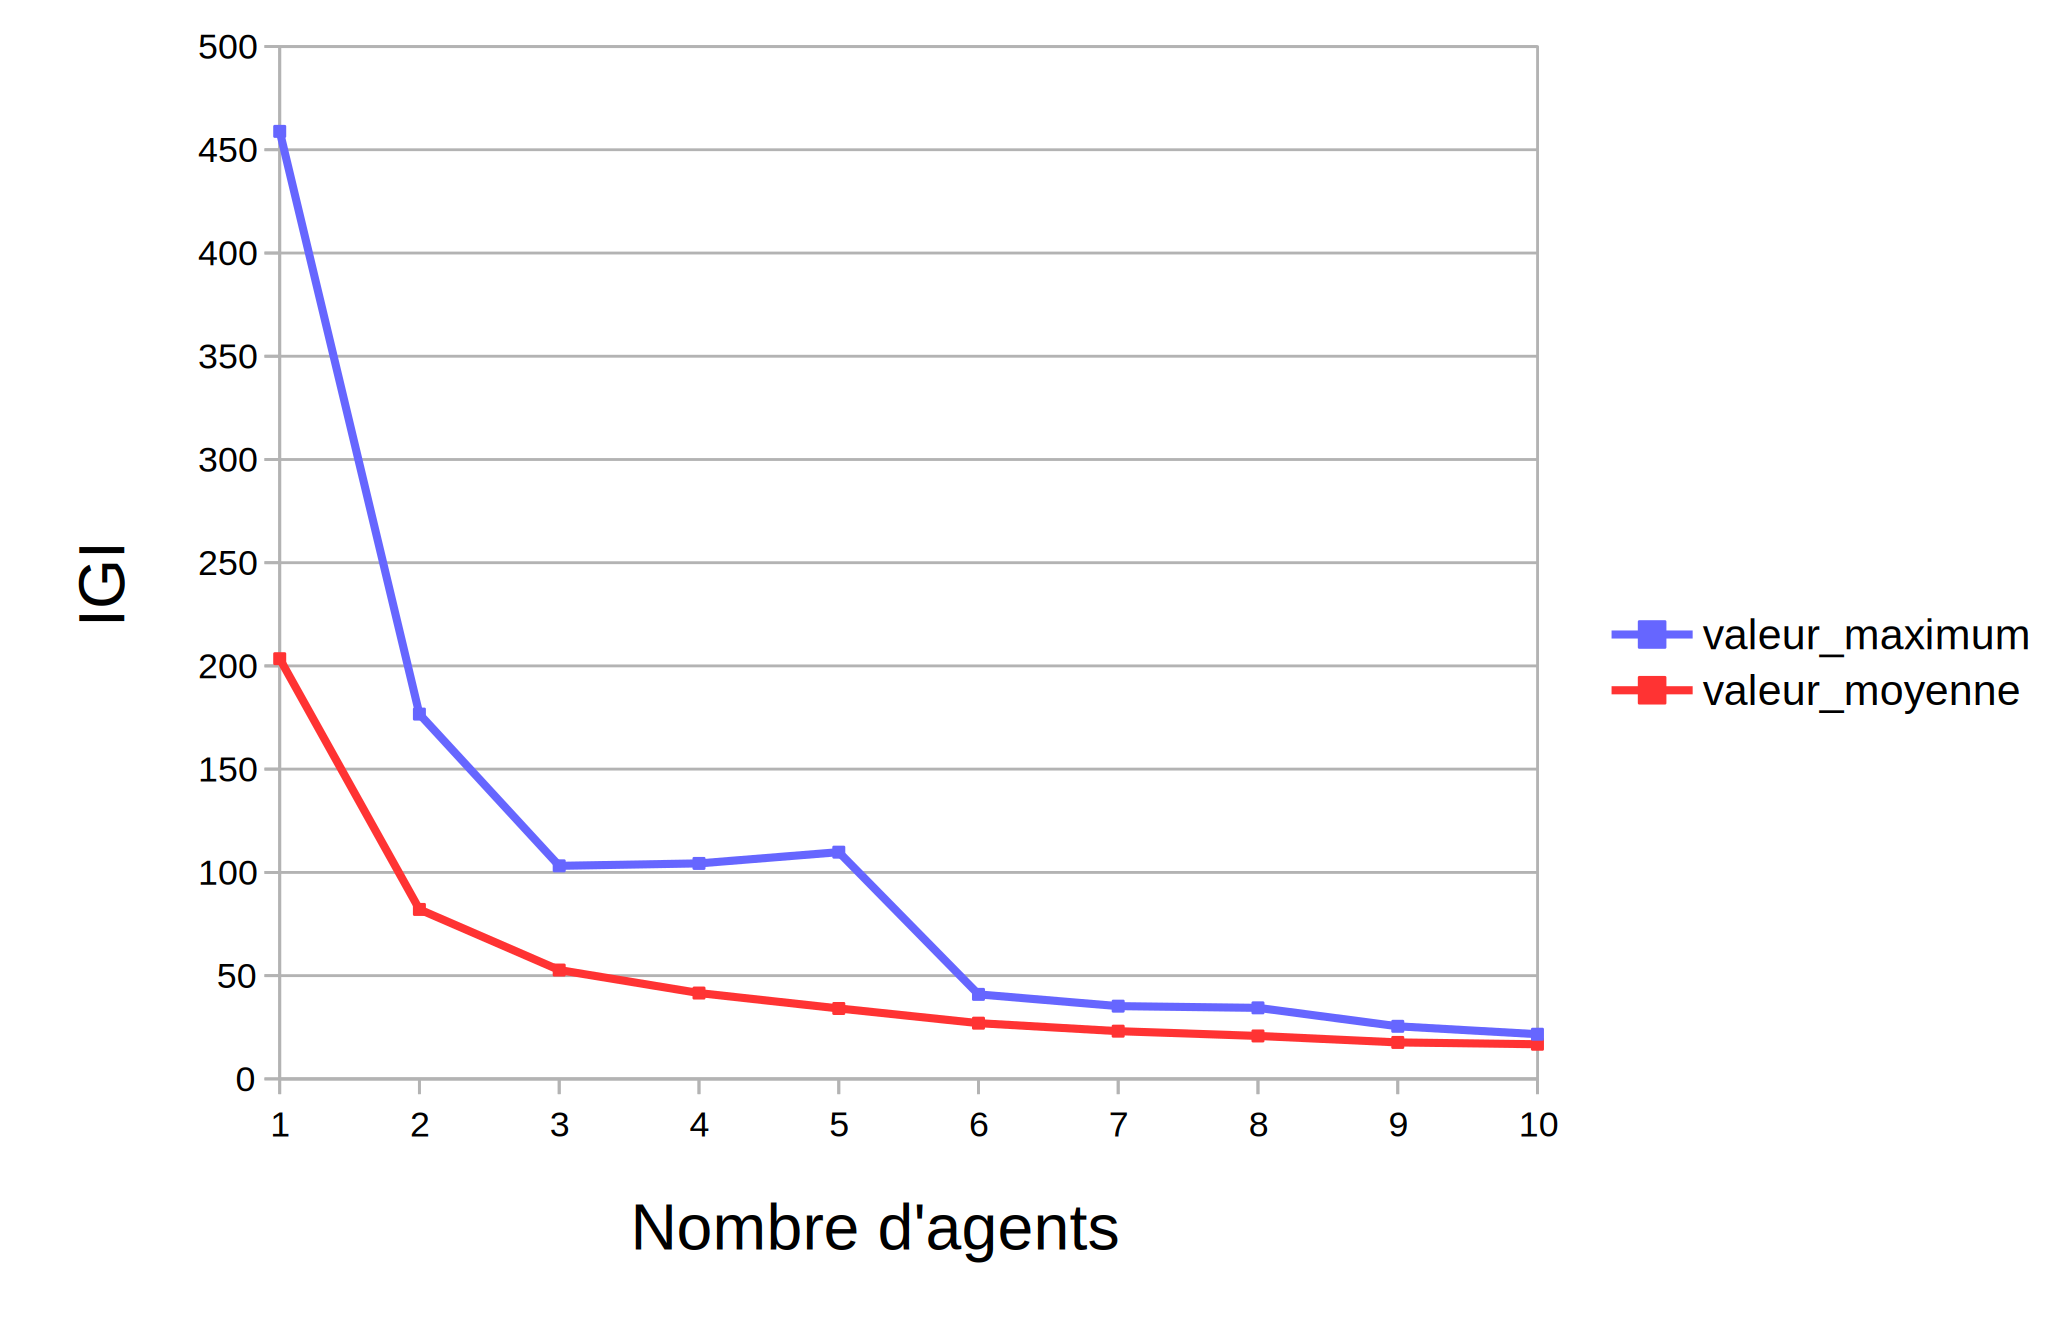
\includegraphics[width = \textwidth]{graphes pdf/variance tortues IGI spirale.pdf}
    \end{center}
    \subsection{Probabilité d'aller tout droit}
\section{Conclusion}
    \subsection{}

\appendix
\newpage
\section{Récapitulatif des types et fonctions}


\end{document}